\documentclass[journal,12pt,twocolumn]{IEEEtran}
\usepackage{amsmath,amssymb,amsfonts,amsthm}
\usepackage{txfonts}
\usepackage{tkz-euclide}
\usepackage{listings}
\usepackage{gvv}
\usepackage[latin1]{inputenc}
\usepackage{array}
\usepackage{pgf}
\usepackage{lmodern}

\begin{document}
\bibliographystyle{IEEEtran}

\title{GATE 2023[IN]-36}
\author{EE23BTECH11066 - Yakkala Amarnath Karthik}
\maketitle
\bibliographystyle{IEEEtran}
\textbf{Question:}\\ \\
The impulse response of an LTI system is $h\brak{t}$= $\delta\brak{t}$+0.5$ \delta\brak{t-4}$, where $\delta\brak{t}$ is continuous-time unit impulse signal.if the input signal $x(t)=\cos\brak{\frac{7\pi t}{4}}$,the output is\hfill(GATE IN 2023)\\ \\

\textbf{Solution:}\\
\begin{table}[ht]
 \centering
  \begin{tabular}{|c|c|c|}
    \hline
    \textbf{Variable} & \textbf{Description} & \textbf{value}\\
    \hline
    $\delta\brak{t}$ & continuous-time unit impulse signal & 1 if t=0;\\ & &  0 in other cases\\
   \hline
    $h\brak{t}$ & impulse response & $\delta\brak{t}$+0.5$ \delta\brak{t-4}$ \\
    \hline
    $x\brak{t}$ & input signal  & $x(t)=cos\brak{\frac{7\pi t}{4}}$ \\
    \hline
    $y\brak{t}$ & output signal & x\brak{t}$ *$ h\brak{t} \\
    \hline
     $\mathcal{F}\brak{\cos{\omega_0 t}}$ & Fourier transform of $\cos{\omega t}$ & $\pi \sbrak{\delta \brak{\omega - \omega_0}+ \delta \brak{\omega + \omega_0}}$\\
    \hline
    $Y\brak{f}$ &  Fourier transform of $y\brak{t}$ & 0.5$\pi \sbrak{\delta \brak{\omega - \frac{7\pi}{4}}+ \delta \brak{\omega + \frac{7\pi}{4}}}$\\
    \hline
    $X\brak{f}$ & Fourier transform of $x\brak{t}$ & $\pi \sbrak{\delta \brak{\omega - \frac{7\pi}{4}}}+ \delta \brak{\omega + \frac{7\pi}{4}}$\\
    \hline
    \end{tabular}
  \caption{A Table with input parameters}
  \label{tab:gate2023in36}
\end{table}
\\
from \tabref{tab:gate2023in36}
\begin{align}
    &Y\brak{f} = X\brak{f}H\brak{f}\\
   % &= \sbrak{1+0.5e^{-j8\pi f}}\sbrak{\pi \sbrak{\delta \brak{2\pi f - \frac{7\pi}{4}}}+ \delta \brak{2\pi f + \frac{7\pi}{4}}}\\
   &=0.5\sbrak{\delta \brak{f-\frac{7}{8}}+\delta \brak{f+\frac{7}{8}}}\sbrak{1+0.5e^{-j8\pi f}}
 % Suppress equation numbering for this line
\end{align}

Finding inverse fourier transform of Y$\brak{f}$:
\begin{align}
    y\brak{t}&=\int_{-\infty}^{\infty}Y\brak{f}e^{j2\pi ft}df\\
    &=0.5\cos\brak{{\frac{7\pi t}{4}}}
\end{align}


  \begin{figure}[ht]
        \hspace{3cm} \\ \\ \\ \\ \\ \\ \\ 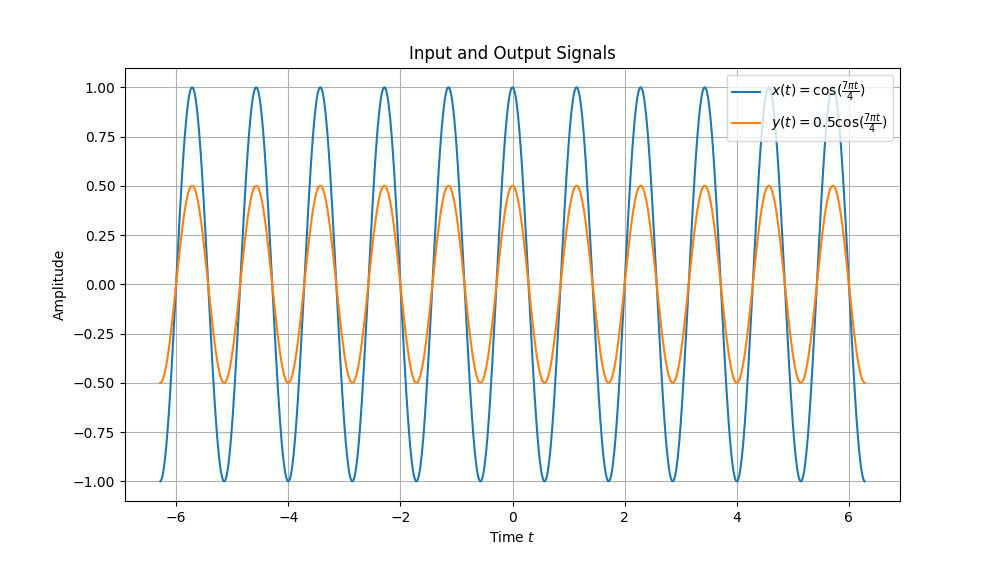
\includegraphics[width=0.45\textwidth]{figs/pythongate.png}
        \caption{Graph showing x(t) and y(t)}
    \end{figure} 

\end{document}

